\chapter{CNN I}
\section{Neural Networks}
An Artificial Neural Network is a system consisting of interconnected units that compute nonlinear functions.
\begin{itemize}
    \item \textbf{input} units represent input variables.
    \item \textbf{output} units represent output variables.
    \item \textbf{hidden} units represent internal variables that codify (after learning) correlations among input and desired output variables.
    \item \textbf{weights} are associated to connections between units.
\end{itemize}
Multiple layers of cascaded units makes a Neural Network able to implement complex non linear functions. The non linearity of the model is given by the activation functions. In fact, without them (linear activation) the result of the model, even if it’s very complex, would still be linear.
\begin{itemize}
    \item \textbf{Sigmoid:}
    \[\frac{1}{1 + e^{-y}}\]

    \item \textbf{ReLU:}
    \[max(0, y)\]
    
    \item \textbf{tanh:}
    \[tanh(x)\]

    \item \textbf{Leaky ReLU:}
    \[max(0.1x, x)\]
\end{itemize}
The basic idea of the learning algorithm consists in two phases:
\begin{itemize}
    \item \textbf{Forward phase:} for each example in the training set, present it to the network and compute the output. Each neuron performs a dot-product with the input and its weights, adds the bias and applies the \textbf{activation function}.
    
    \item \textbf{Backward phase:} Back-propagate the committed error and update the weights of the hidden units accordingly. 
\end{itemize}
\textbf{Back-propagation} is an algorithm based on the gradient descent method that aims to update the weights of a Neural Network in order to minimize the error between the predicted output and the true output. The algorithm works by propagating the error back through the network, starting with the output layer and moving backwards through the hidden layers, adjusting the weights at each layer to reduce the error. It can be implemented in different ways:
\begin{itemize}
    \item \textbf{Batch gradient descent:} It \textbf{cumulates} gradients over all the training examples and then updates the weights.
    \item \textbf{Stochastic gradient descent:} For each example in $S$, it computes the gradients and update the weights.
    \item \textbf{Mini-batch gradient descent:} It updates the weights considering a subset of examples $Q \subseteq S$. 
\end{itemize}
This process is typically repeated many times until the error is sufficiently small or the maximum number of iterations is reached. Let's define the algorithm according to the derivations seen before:

\section{Convolutional Networks}
Convolutional networks, also known as convolutional neural networks or CNNs, are a specialized kind of neural network for processing data that has a known, grid-like topology. Examples include time-series data, which can be thought of as a 1D grid taking samples at regular time intervals, and image data, which can be thought of as a 2D grid of pixels. Convolutional networks have been tremendously successful in practical applications. The name “convolutional neural network” indicates that the network employs a mathematical operation called convolution. The idea is to substitute matrix multiplication with convolution.\newline\newline
Images have three properties that suggest the need for specialized architecture:
\begin{itemize}
    \item they are high-dimensional, e.g. 224×224 RGB values (i.e., 150,528 input dimensions). Hidden layers in fully connected networks are generally larger than the input size, and so even for a shallow network, the number of weights would exceed 150,528! or 22 billion. Obvious practical problems in terms of the required training data, memory, and computation.

    \item Nearby image pixels are statistically related. Fully connected networks have no notion of “nearby” and treats the relationship between every input equally; if the pixels of the training and test images were randomly permuted in the same way, the network could still be trained with no practical difference.

    \item The interpretation of an image is stable under geometric transformations. An image of a tree is still an image of a tree if we shift it leftwards by a few pixels. However, this shift changes every input to the network, and so the model would have to learn the patterns of pixels that correspond to a tree separately at every position. This is clearly inefficient.
\end{itemize}
Convolutional networks are perhaps the greatest success story of biologically
inspired artificial intelligence. Neurophysiologists
David Hubel and Torsten Wiesel collaborated for several years to determine many of the most basic facts about how the mammalian vision system works. They observed how neurons in the cat’s brain responded to images projected
in precise locations on a screen in front of the cat. Their great discovery was that neurons in the early visual system responded most strongly to very specific patterns of light, such as precisely oriented bars, but responded hardly at all to other patterns.

\subsection{Convolution operator}
In its most general form, \textbf{convolution} is an operation on two functions of a real-valued argument. To motivate the definition of convolution, we start with examples of two functions we might use.\newline\newline
Suppose we are tracking the location of a spaceship with a laser sensor. Our
laser sensor provides a single output $x(t)$, the position of the spaceship at time $t$. Both $x$ and $t$ are real-valued, i.e., we can get a different reading from the laser sensor at any instant in time.\newline\newline
Now suppose that our laser sensor is somewhat noisy. To obtain a less noisy
estimate of the spaceship’s position, we would like to average together several measurements. Of course, more recent measurements are more relevant, so we will want this to be a weighted average that gives more weight to recent measurements. We can do this with a weighting function $w(a)$, where $a$ is the age of a measurement. If we apply such a weighted average operation at every moment, we obtain a new function $s$ providing a smoothed estimate of the position of the spaceship:

\[s(t) = \int_{-\infty}^{\infty} x(a)w(t - a)da\]
The convolution operation is typically denoted with an asterisk:
\[s(t) = (x \,*\, w)(t)\]
In convolutional network terminology, the first argument (in this example, the function $x$) to the convolution is often referred to as the \textbf{input} and the second argument (in this example, the function $w$) as the \textbf{kernel} (needs to be a valid probability density function). The output is sometimes referred to as the \textbf{feature map}.\newline\newline
Usually, when we work with data on a computer, time will be discretized:
\[s(t) = (x \,*\, w)(t) = \sum_{a = - \infty}^{\infty}x(a)w(t-a)\]
In machine learning applications, the input is usually a multidimensional array of data and the kernel is usually a multidimensional array of parameters that are adapted by the learning algorithm.\newline\newline
We often use convolutions over more than one axis at a time. For
example, if we use a two-dimensional image $I$ as our input, we probably also want to use a two-dimensional kernel $K$:
\[S(i, j) = (I \, *\, K)(i, j) = \sum_{a = -m}^{m}\sum_{b = -n}^{n}K(a, b)I(i - a, j - b)\]
\begin{center}
    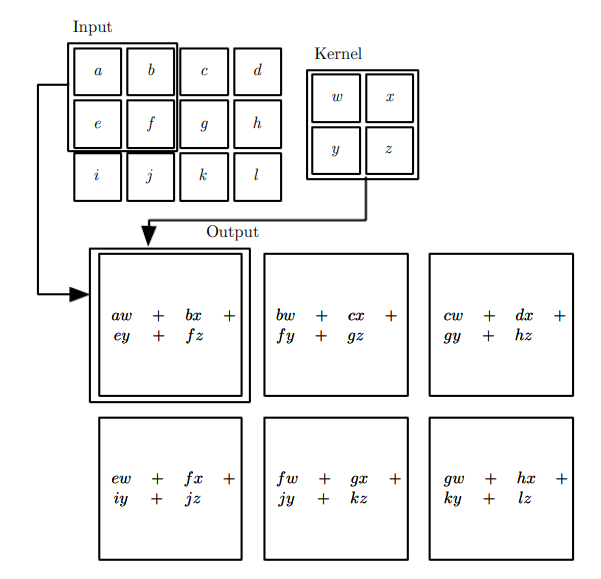
\includegraphics[scale=0.7]{images/Cross-corr.png}
\end{center}
From the example above we can notice two things:
\begin{itemize}
    \item The kernel is applied as a sliding window across the image.

    \item Actually, the operator applied in the example is not convolution, but \textbf{cross-correlation:}
    \[S(i, j) = \sum_{a = -m}^{m}\sum_{b = -n}^{n}K(a, b)I(i + a, j + b)\]
    In fact, we apply convolution by \textbf{flipping} the kernel relative to the input, in the sense that as $b$ increases, the index into the input decreases, but the index into the kernel increases. Many machine learning libraries implement cross-correlation but call it convolution.
\end{itemize}
The main properties of convolution are:
\begin{itemize}
    \item Sparse interactions $\rightarrow$ kernel smaller than input, efficiency.

    \item Parameter sharing

    \item Equivariant representations

    \item Works with inputs of variable size
\end{itemize}

\subsection{Sparse interactions}
Traditional neural network layers use matrix multiplication, having a matrix of parameters with a separate parameter describing the interaction between each input unit and each output unit. Convolutional networks, however, typically have sparse interactions (also referred to as sparse connectivity or sparse weights). This is accomplished by making the kernel smaller than the input. This means that we need to store fewer parameters, which both reduces the
memory requirements of the model and improves its statistical efficiency. It also means that computing the output requires fewer operations.
\begin{center}
    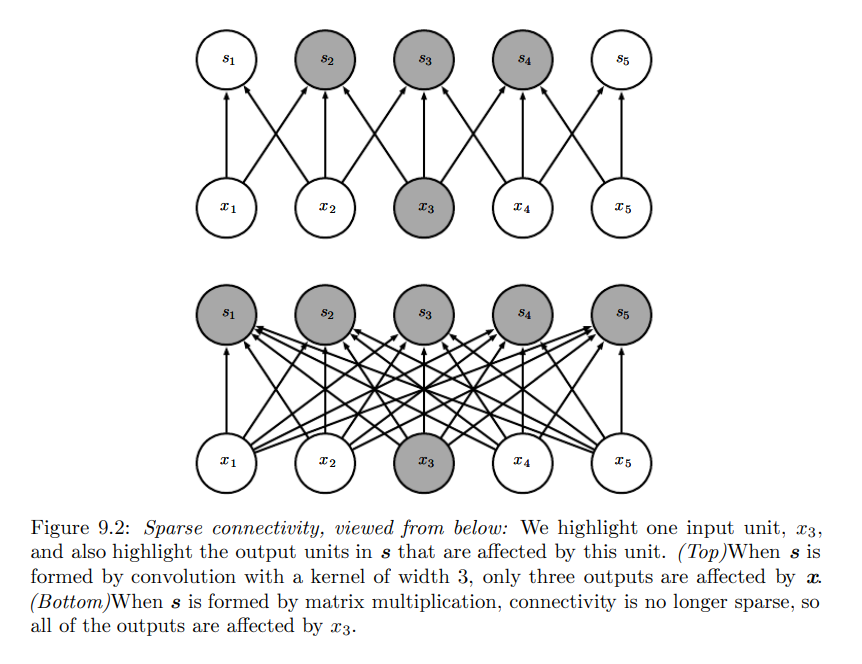
\includegraphics[scale = 0.7]{images/Sparse-conn.png}
\end{center}
The receptive field of the units in the deeper layers of a convolutional network is larger than the receptive field of the units in the shallow layers. This means that even though direct connections in a convolutional net are very sparse, units in the deeper layers can be indirectly connected to all or most of the input. This allows the network to efficiently describe complicated interactions between many variables by constructing such interactions from simple building blocks that each describe only sparse interactions.
\begin{center}
    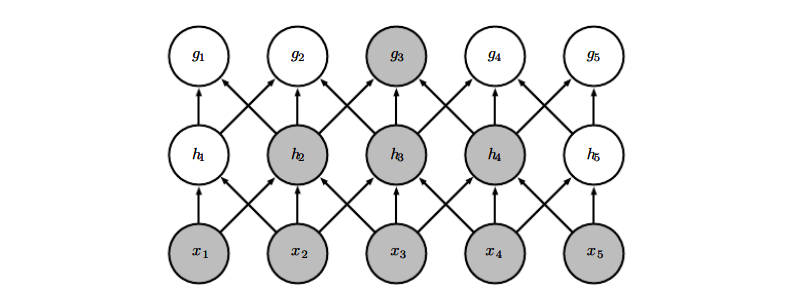
\includegraphics[scale=0.7]{images/receptive field.png}
\end{center}

\subsection{Parameter sharing}
\textbf{Parameter sharing} refers to using the same parameter for more than one function in a model. In a traditional neural net, each element of the weights' matrix is used exactly once when computing the output of a layer. In a convolutional neural net, each member of the kernel is used at every position of the input (except perhaps some of the boundary pixels, depending on the design decisions regarding the boundary). The parameter sharing used by the convolution operation means that rather than learning a separate set of parameters for every location, we learn only one set. It further reduces the storage requirements of the model to $k$ parameters (just the filter), with $k$ several order of magnitude smaller than the input size. Convolution is thus dramatically more efficient than dense matrix multiplication in terms of the memory requirements and statistical efficiency.
\begin{center}
    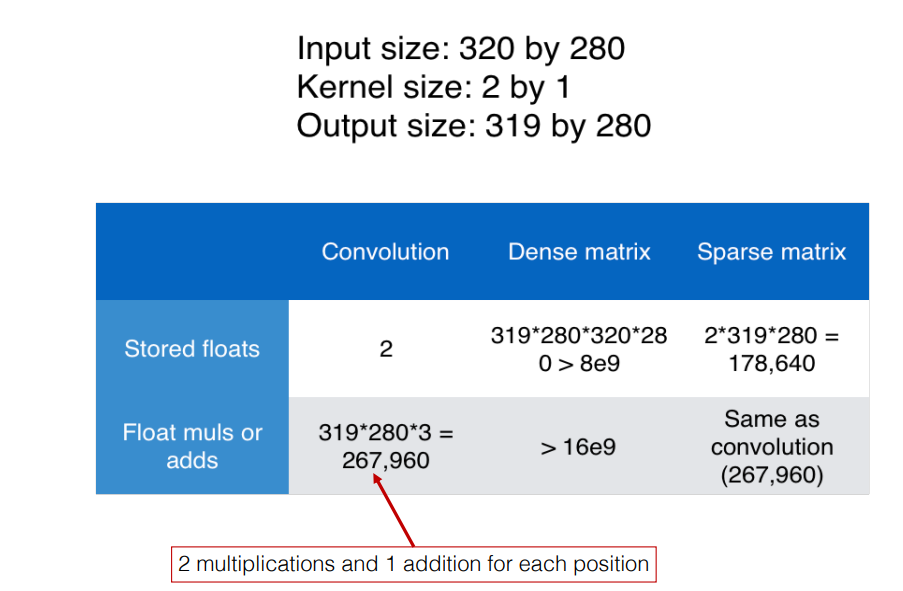
\includegraphics[scale=0.7]{images/conv-efficiency.png}
\end{center}

\subsection{Equivariance to translation}
In the case of convolution, the particular form of parameter sharing causes the layer to have a property called \textbf{equivariance} to translation. To say a function is
equivariant means that if the input changes, the output changes in the same way. Specifically, a function $f(x)$ is equivariant to a function $g$ if $f(g(x)) = g(f(x))$. In the case of convolution, if we let $g$ be any function that translates the input, i.e., shifts it, then the convolution function is equivariant to $g$. For example, with images, convolution creates a 2-D map of where certain features appear in the input. If we move the object in the input, its representation will move the
same amount in the output. Basically, due to parameter sharing, the kernel detects a feature regardless of where the feature is in the input image.\newline\newline
Convolution is not naturally equivariant to some other transformations, such as changes in the scale or rotation of an image. Other mechanisms are necessary for handling these kinds of transformations.

\subsection{Inputs of variable size}
Consider a collection of images, where each image has a different
width and height. It is unclear how to model such inputs with a weight matrix of fixed size. Convolution is straightforward to apply; the kernel is simply applied a different number of times depending on the size of the input, and the output of the convolution operation scales accordingly.

\subsection{Strided Convolution}
We may want to skip over some positions of the kernel in order to reduce the
computational cost (at the expense of not extracting our features as finely).
We can think of this as downsampling the output of the full convolution function. We can do this by sampling only every $s$ pixels in each direction in the output. We refer to $s$ as the \textbf{stride} of this downsampled convolution. It is also possible to define a separate stride for each direction of motion.
\begin{center}
    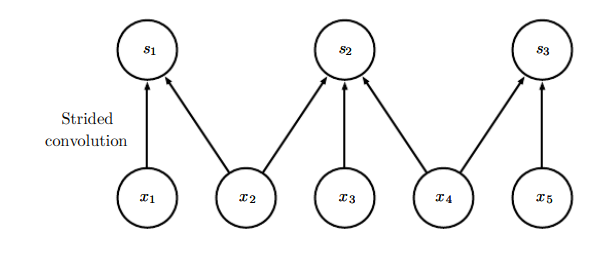
\includegraphics[scale=0.7]{images/stride.png}
\end{center}

\subsection{Dilated Convolution}
Increasing the kernel size has the disadvantage of requiring more weights. In order to reduce the number of stored weights we can use \textbf{dilated convolution}, that is, the kernel values are spaced with zeros. In 1D we can turn a kernel of size five into a dilated kernel of size three by setting the second and fourth elements to zero. We still integrate information from a larger input region but only require three weights to do this. The number of zeros we intersperse between the weights is termed the dilation rate.

\subsection{Pooling}
A typical layer of a convolutional network consists of three stages. In the first stage, the layer performs several convolutions in parallel to produce a set of linear activations. In the second stage, each linear activation is run through a nonlinear activation function, such as the rectified linear activation function. In the third stage, we use a pooling function to modify the output of the layer further.\newline\newline
A pooling function replaces the output of the net at a certain location with a summary statistic of the nearby outputs. For example, the \textbf{max pooling} operation reports the maximum output within a rectangular neighborhood. Another popular pooling function is the average of a rectangular neighborhood.
\begin{center}
    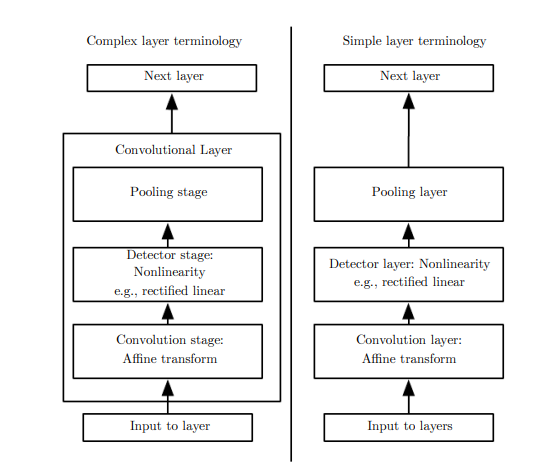
\includegraphics[]{images/cnn-structure.png}
\end{center}
In all cases, pooling helps to make the representation become approximately invariant to small translations of the input. Invariance to translation means that if we translate the input by a small amount, the values of most of the pooled outputs do not change. Furthermore, pooling reduces the size of the input of the subsequent layers, thus it improves efficiency.\newline\newline
For many tasks, pooling is essential for handling inputs of varying size.

\subsection{Padding}
Given an $n \times n$ kernel, its external row/column coincides with the border of the image when the center of this mask is at distance $\frac{n-1}{2}$ from the edge. If you move further out, part of the window \textit{leaves} the image.\newline
This situation can be managed in three different ways:
\begin{itemize}
    \item limit the movement of the mask, keeping it at a minimum distance of $\frac{n-1}{2}$ from the edges.
    \item duplicate the external rows/columns of the image
    \item enlarge the image with rows/columns of zeros
\end{itemize}
Solution 1 gives reliable results, but produces a different size image from the original. Solutions 2 and 3, on the other hand, give results that are not exactly authentic near the edges, but are often convenient because they allow you to obtain an output image with the same size as the input one.

\subsection{Multi-channel input}
\begin{center}
    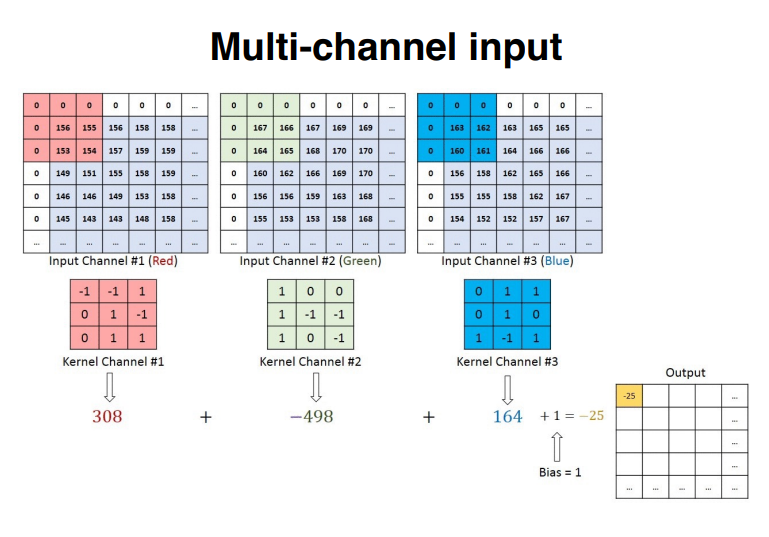
\includegraphics[]{images/multi-channel input.png}
\end{center}


\subsection{Unshared convolution}
In some cases, we do not actually want to use convolution, but rather locally connected layers. This is sometimes also called \textbf{unshared convolution}, because it is a similar oper- ation to discrete convolution with a small kernel, but without sharing parameters across locations. Locally connected layers are useful when we know that each feature should be
a function of a small part of space, but there is no reason to think that the same feature should occur across all of space.

\subsection{Structured Outputs}
Convolutional networks can be used to output a high-dimensional, structured
object, rather than just predicting a class label for a classification task or a real value for a regression task. Typically, this object is a tensor with the same shape of the input, with a class label for each pixel to produce object detection masks.
